<<<<<<< HEAD
As a first step, the susceptibility of an Ising lattice was examined as can be seen in Figure (\ref{fig:results_isingsusc}). This is done by measuring the average number of steps taken from each loop in the Worm algorithm. This corresponds to sampling the correlation function, that is related to the susceptibility as $\chi \propto \sum G_{ij}$, where $G_{ij}$ is the correlation function between site $i$ and $j$.

=======
>>>>>>> cc146c4b0c95168aaa889d3303a457ca393fed00

\begin{figure}[h!]
    \centering
        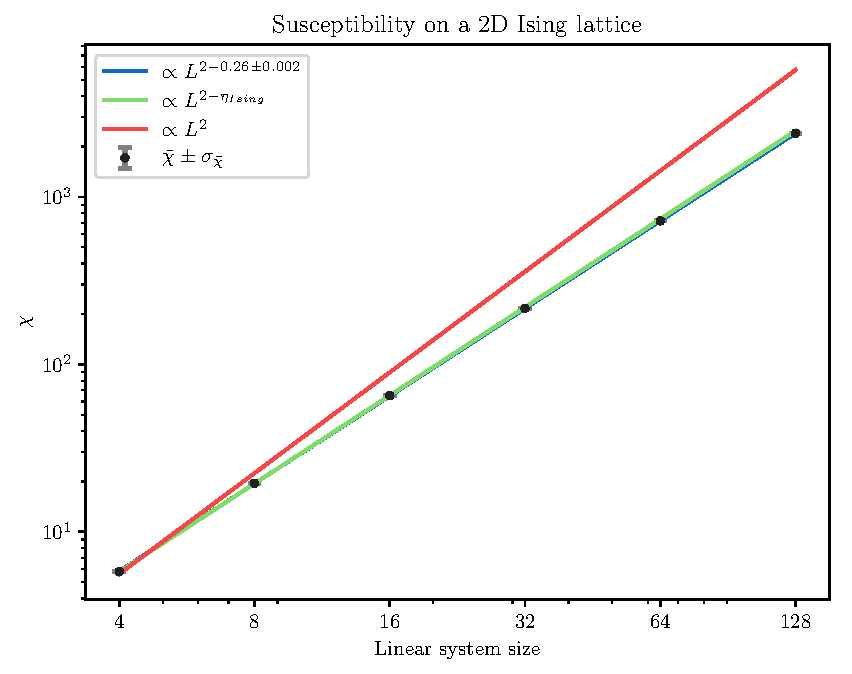
\includegraphics[width=0.8\textwidth]{figures/susceptibility128x128Ising.pdf}
    \caption{Scaling of susceptibility at $T_c$ on an Ising lattice of varying sizes. The measured critical exponent $\eta = 0.26 \pm 0.002$ is compared to the theoretical value $\eta_{Ising} = 0.25$ \cite{Plischke:EqStatMech}. The red line labeled $\propto L^2$ illustrates data where susceptibility scales with system size.}
    \label{fig:results_isingsusc}
\end{figure}

<<<<<<< HEAD

\noindent Sampling this correlation function is done for a sequence of different system sizes, $L = 2^n = 4, \ 8, \ 16, \ \ldots, \ 128$, and with the critical temperature $T_c$. According to the scaling hypothesis \cite{Plischke:EqStatMech}, the expected scaling exponent for the Ising susceptibility is $\eta_{Ising} = 0.25$, and is computed here to be $\eta = 0.26 \pm 0.002$.

Figure (\ref{fig:results_boxdimension}) displays the box dimension of the largest cluster on a $128^3$ Ising cluster. The largest cluster is found by first labeling all clusters with the Hoshen Kopelman algorithm, and then isolating the one with the largest number of links. The graph is then divided into a set of boxes with decreasing sidelength, as showed in the x-axis of Figure (\ref{fig:results_boxdimension}). The box dimension is then calculated as

\begin{equation}
    d = \lim_{\epsilon \to 0} \frac{\ln N(\epsilon)}{\ln 1 / \epsilon}
\end{equation}

where $N(\epsilon)$ is the number of boxes needed to cover the cluster. The green line shows the theoretical value for these clusters as $D_H = 1.375$ \cite{Duplantier:GeoHausdorff}, and is computed here to be $D_H = 1.35193 \pm 5 \cdot 10^{-4}$.

=======
>>>>>>> cc146c4b0c95168aaa889d3303a457ca393fed00
\begin{figure}[h!]
    \centering
        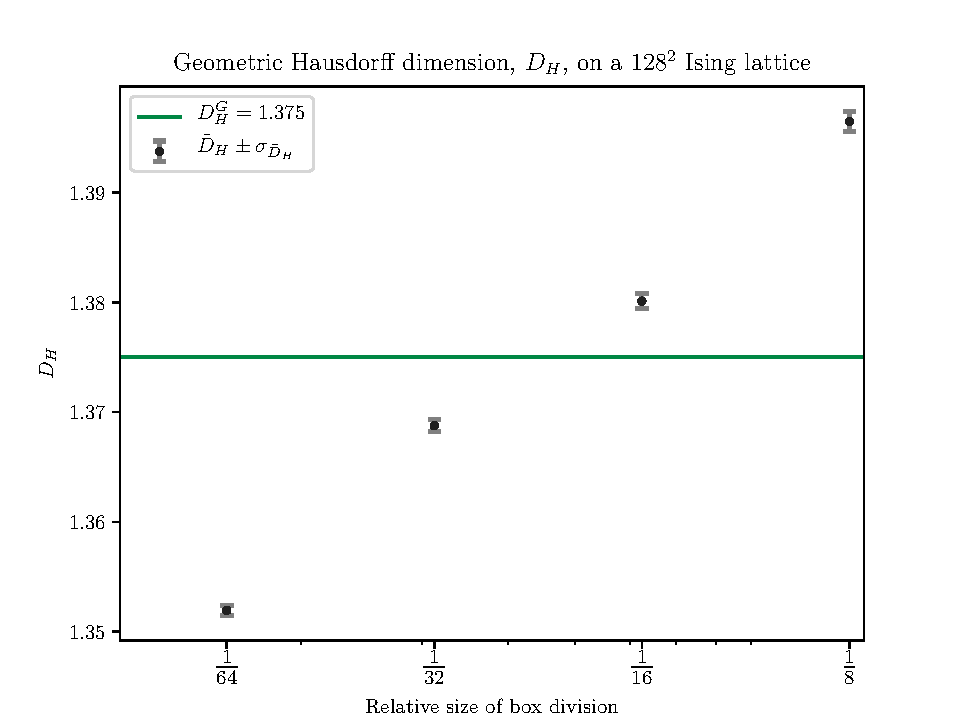
\includegraphics[width=0.8\textwidth]{figures/box_dim_128x128Ising.pdf}
    \caption{Hausdorff dimension of the maximum loop length on a $128^2$ Ising lattice at $T_c$ using the box dimension. The $x$ axis shows the size of one box relative to the side length of the lattice. The green line indicates the theoretical dimension of the geometric Ising cluster, $D_H^G = 1.375$ \cite{Duplantier:GeoHausdorff}. Comparing to the smallest box size as $D_H = 1.35193 \pm 5 \cdot 10^{-4}$.}
    \label{fig:results_boxdimension}
\end{figure}

<<<<<<< HEAD
\newpage

A similar approach is used in Figure (\ref{fig:results_maxloopdimension}), where the scaling dimension of the largest cluster is examined. The largest cluster in terms of number of links is determined over a sequence of system sizes at $T_c$. This is then fitted to produce a scaling exponent of $D_H = 1.38 \pm 0.02$ compared to the theoretical value $D_H^G = 1.375$ \cite{Duplantier:GeoHausdorff}.


=======
>>>>>>> cc146c4b0c95168aaa889d3303a457ca393fed00
\begin{figure}[h!]
    \centering
        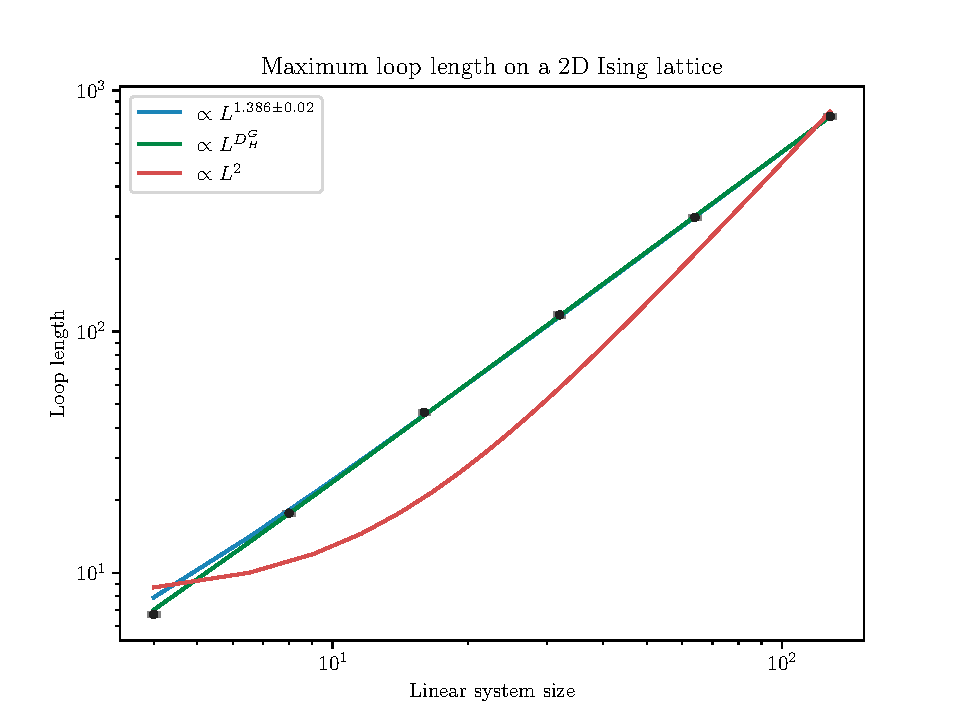
\includegraphics[width=0.8\textwidth]{figures/maximum_loop_length_for_2D_Ising.pdf}
    \caption{Log-log plot of the maximum loop length at $T_c$ on an Ising lattice of varying sizes. The measured scaling factor is $1.38 \pm 0.02$ compared to the theoretical Hausdorff dimension, $D_H^G = 1.375$ \cite{Duplantier:GeoHausdorff}. The red line labeled $\propto L^2$ illustrates data where maximum loop length scales with system size.}
    \label{fig:results_maxloopdimension}
\end{figure}

<<<<<<< HEAD
\newpage

Figure (\ref{fig:comparsion_2d_lattice_dimensions}) displays a comparison between the two methods showed in Figures (\ref{fig:results_boxdimension}-\ref{fig:results_maxloopdimension}) together with the dimensions of random and self avoiding walks. The dimensions computed with the scaling and the box counting method show that the shape of the Ising cluster is similar to that of the self avoiding walk. This can be seen further by examining Figure (\ref{fig:largest_cluster_illu}), where an isolated largest cluster on a $128^2$ Ising lattice is shown.

=======
>>>>>>> cc146c4b0c95168aaa889d3303a457ca393fed00
\begin{figure}[h!]
    \centering
        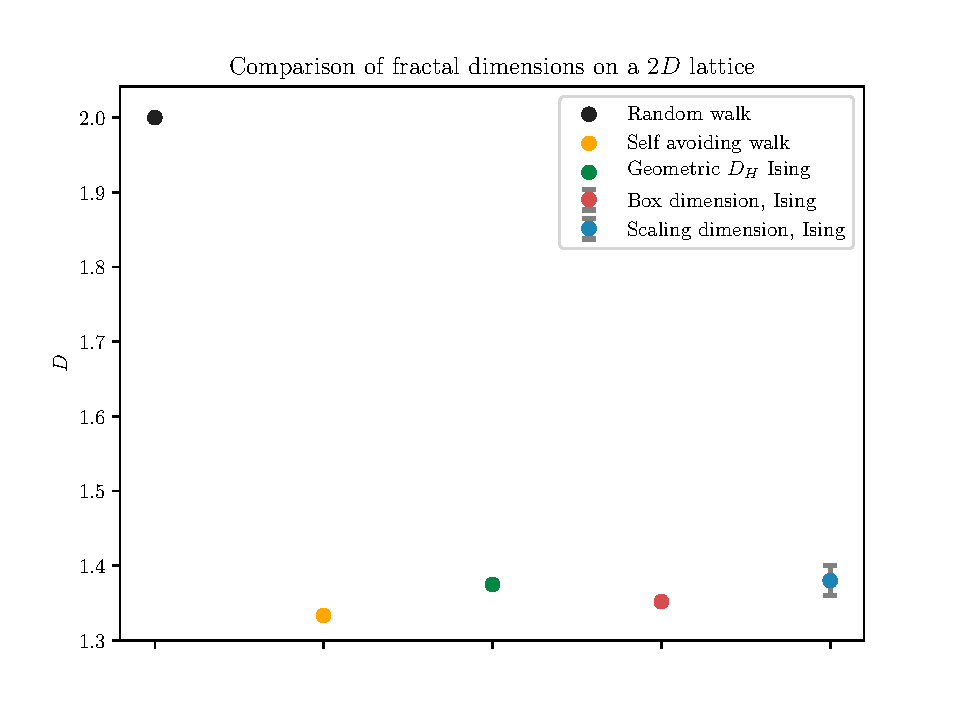
\includegraphics[width=0.8\textwidth]{figures/dimenson_comparison.pdf}
    \caption{Comparison between different algorithms and ways of calculating the fractal dimension on a $2D$ lattice. The random walk has a dimension of $2$, the self avoiding walk has $4/3$ \cite{Vilgis:FlorySAW}. The geometric Hausdorff dimension has an exact value of $1.375$ \cite{Duplantier:GeoHausdorff}. This is then approximated using the worm algorithm and calculated using both the box counting method and the scaling dimension method explained in Section \ref{subsec:ScalingDimension}.}
    \label{fig:comparsion_2d_lattice_dimensions}
\end{figure}

<<<<<<< HEAD
\newpage

\noindent The difference between the self avoiding walk and the Ising cluster is that the Worm algorithm allows the path to cross itself, creating a structure ressembling `twisted loops' as can be seen in Figure (\ref{fig:largest_cluster_illu}). This might indicate a new type of self avoiding loop, where self crossing is allowed.
=======
>>>>>>> cc146c4b0c95168aaa889d3303a457ca393fed00

\begin{figure}[h!]
    \centering
        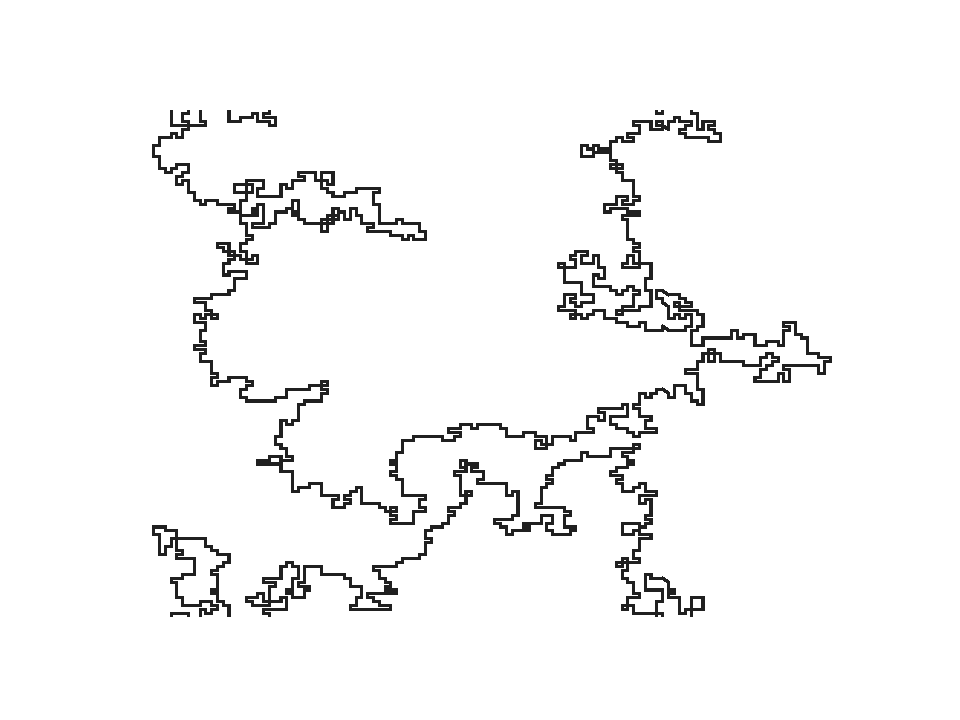
\includegraphics[width=0.8\textwidth]{figures/largest_cluster_testing_nolattice.pdf}
    \caption{Isolated largest cluster on a $128^2$ Ising lattice with periodic boundary conditions.}
    \label{fig:largest_cluster_illu}
\end{figure}

<<<<<<< HEAD
\newpage

Next, the XY model was examined. To simplify the algorithm, the Villain approximation \cite{Villain:VillainOriginalPaper} was used. This gives a new expression for the energy as

\begin{equation}
    E = \frac{1}{2} \sum_i J^2_i
\label{eq:results_villain_energy}
\end{equation}

where $J_i$ is the flux associated with site $i$. However, in this approximation, the critical temperature is shifted due to the fact that the acceptance probability is changed by the new expression of the energy. One way of determining the new critical temperature is to measure the superfluid density, as it should fall to zero as the temperature is shifted from above, to below $T_c$. This is done by measuring the winding number, as it relates to the superfluid density as

\begin{equation}
    \langle W^2 \rangle \propto \frac{L}{T} \rho_s
\end{equation}

for a $3D$ XY lattice. Figure (\ref{fig:results_windingnumberTc}) show the overall structure of the average winding number squared, plotted for a range of system sizes and temperatures.

=======
>>>>>>> cc146c4b0c95168aaa889d3303a457ca393fed00
\begin{figure}[h!]
    \centering
        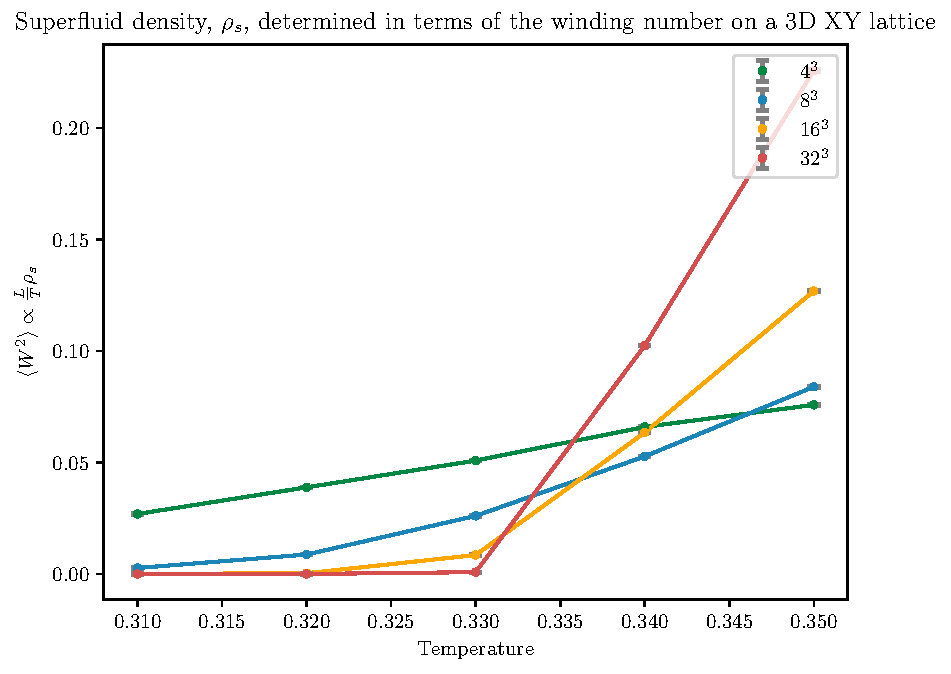
\includegraphics[width=0.8\textwidth]{figures/winding_number_Tc.pdf}
    \caption{Average winding number squared, $\langle W^2 \rangle \propto \rho_s$, plotted on a 3D XY lattice of varying sizes. The overall structure of the average winding number squared as a function of the temperature is shown.}
    \label{fig:results_windingnumberTc}
\end{figure}

<<<<<<< HEAD
\newpage

The intersection between all system sizes of average winding number squared is then determined in Figure (\ref{fig:results_windingnumberTcZoomed}). The inset, together with the red line shows $T_c = 0.3331 \pm 1 \cdot 10^{-4}$ taken as the weighted average of all intersections with the system sizes as weights. Note here that the temperature in the Villain approximation goes as one over the real temperature \cite{Villain:VillainOriginalPaper}, giving a non-zero superfluid density for high `temperature'.
=======
>>>>>>> cc146c4b0c95168aaa889d3303a457ca393fed00

\begin{figure}[h!]
    \centering
        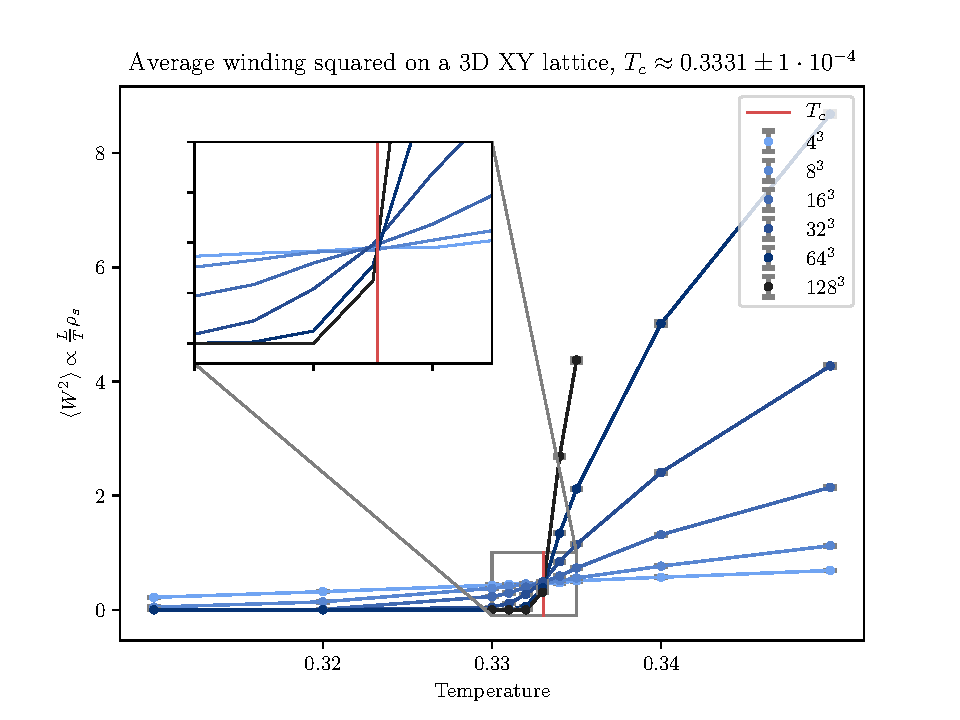
\includegraphics[width=0.8\textwidth]{figures/winding_number_Tc_zoomed.pdf}
    \caption{Average winding number squared, $\langle W^2 \rangle \propto \rho_s$, plotted on a 3D XY lattice of varying sizes. Due to the Villain approximation the transition is flipped such that $\rho_s \neq 0$ for $T > T_c$, and $T_c$ is translated from $\approx 2.2$ \cite{Gottlob:CritBehaviour3DXY} to $\approx 0.333$ indicated by the intersection. By taking the weighted average of the intersections the critical temperature can be estimated to $T_c = 0.3331 \pm 1 \cdot 10^{-4}$.}
    \label{fig:results_windingnumberTcZoomed}
\end{figure}

<<<<<<< HEAD
\newpage

When the critical temperature has been computed, the box counting method can be applied to the XY system. Figure (\ref{fig:results_boxdimension_xy}) displays the Hausdorff dimension as a function of the relative size of the box. The smallest box indicates the most exact value, $D_H = 1.77468 \pm 4 \cdot 10^{-6}$, and is compared to data from Prokof'evs and Svistunovs paper, $D_H^P = 1.7655 \pm 2 \cdot 10^{-3}$ \cite{Prokofev:comment_on_hove_hausdorff_crit_fluct}, and Hove, Mo and Sudbo's paper, $D_H^S = 2.287 \pm 2 \cdot 10^{-3}$ \cite{Hove:hausdorff_crit_fluctuations}.

=======
>>>>>>> cc146c4b0c95168aaa889d3303a457ca393fed00
\begin{figure}[h!]
    \centering
        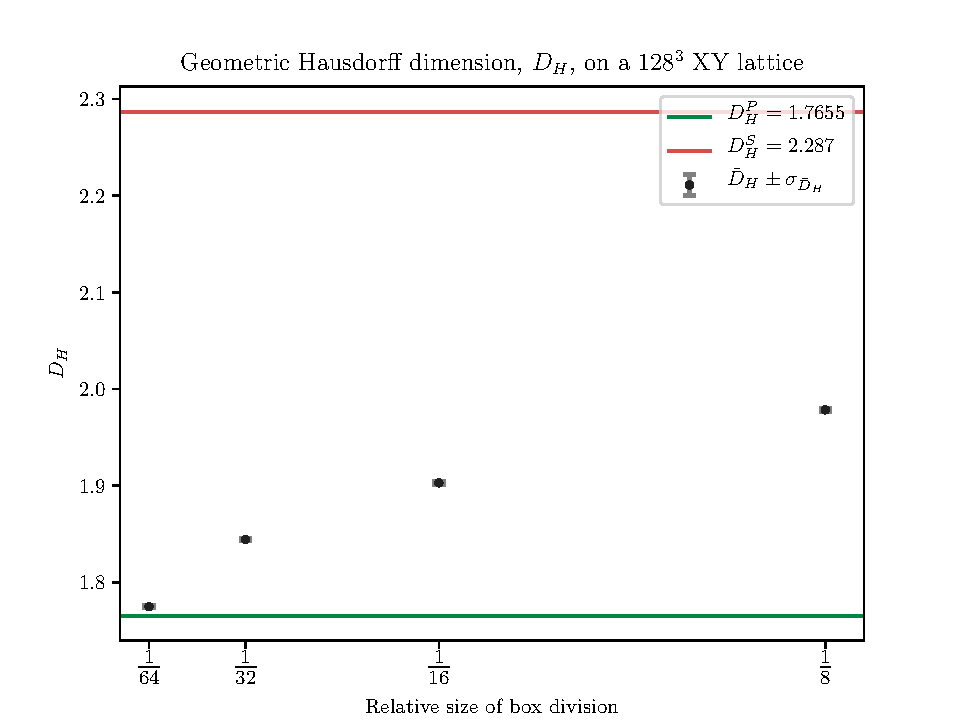
\includegraphics[width=0.8\textwidth]{figures/box_dimension_xy_128x3.pdf}
    \caption{Hausdorff dimension of the maximum loop length on a $128^3$ XY lattice at $T_c$ using the box dimension. The $x$ axis shows the size of one box relative to the side length of the lattice. Assuming that the smallest box size gives the best approximation, the result is $D_H = 1.77468 \pm 4 \cdot 10^{-6}$. This is compared to data from Prokof'evs and Svistunovs paper $D_H^P = 1.7655 \pm 2 \cdot 10^{-3}$ \cite{Prokofev:comment_on_hove_hausdorff_crit_fluct} and Hove, Mo and Sudbo's paper $D_H^S = 2.287 \pm 2 \cdot 10^{-3}$ \cite{Hove:hausdorff_crit_fluctuations}.}
<<<<<<< HEAD
    \label{fig:results_boxdimension_xy}
\end{figure}

\newpage

A comparison without the extra data from the larger box sizes is shown in Figure (\ref{fig:dim_comparison_xy}). The measured dimension from the box counting method closely ressembles that of Prokof'ev and Svistunov.
=======
    \label{fig:results_boxdimension}
\end{figure}

>>>>>>> cc146c4b0c95168aaa889d3303a457ca393fed00

\begin{figure}[h!]
    \centering
        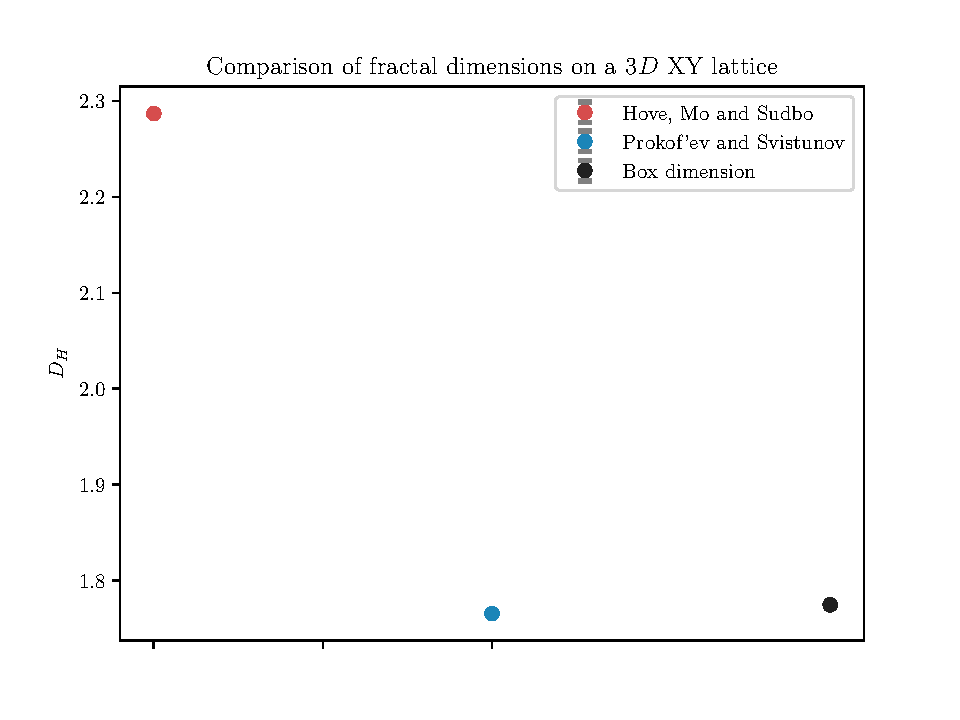
\includegraphics[width=0.8\textwidth]{figures/dimenson_comparison_XY.pdf}
    \caption{Comparison between results from different papers of the Hausdorff dimension of the maximum loop length on a XY lattice at $T_c$. The result from this thesis is labeled `box dimension' and yields the result $D_H = 1.77468 \pm 4 \cdot 10^{-6}$. This is compared to data from Prokof'evs and Svistunovs paper $D_H^P = 1.7655 \pm 2 \cdot 10^{-3}$ \cite{Prokofev:comment_on_hove_hausdorff_crit_fluct} and Hove, Mo and Sudbo's paper $D_H^S = 2.287 \pm 2 \cdot 10^{-3}$ \cite{Hove:hausdorff_crit_fluctuations}.}
    \label{fig:dim_comparison_xy}
\end{figure}

<<<<<<< HEAD
\newpage

Finally, the total energy of the XY lattice is plotted for a sequence of system sizes at $T_c$. The total energy is calculated in the Villain approximation as shown in Equation (\ref{eq:results_villain_energy}). This scaling coefficient of the energy here is $2.91 \pm 0.09$, and is therefore close to scaling as the spatial dimension of the system. This is expected since 

\begin{equation}
    E = L^d ( a t^{1 - \alpha} + b ) \propto L^d, \ \text{at $T = T_c$}
\end{equation}

where $t = T - T_c$, and $a$ and $b$ are some unknown constants.

=======
>>>>>>> cc146c4b0c95168aaa889d3303a457ca393fed00
\begin{figure}[h!]
    \centering
        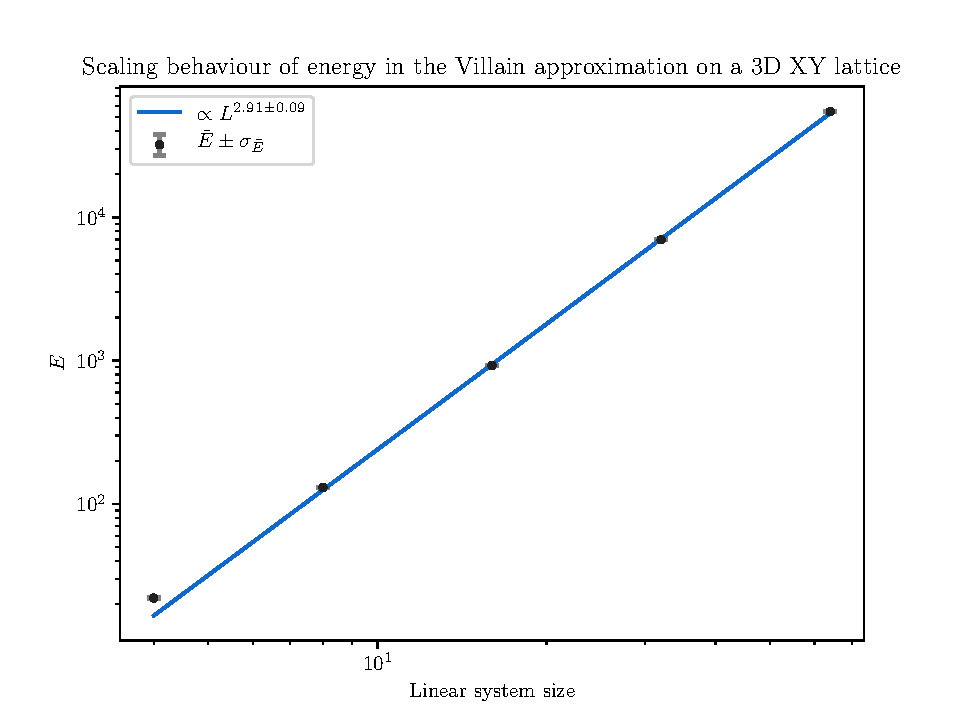
\includegraphics[width=0.8\textwidth]{figures/energy_scaling_xy.pdf}
    \caption{Log-log plot of the energy at $T_c$ on an 3D XY lattice of varying sizes. The measured scaling factor is $2.91 \pm 0.09$. The energy in the Villain approximation is proportional to the sum of the squares of flux flowing through the lattice.}
    \label{fig:results_energyxy}
\end{figure}

<<<<<<< HEAD

=======
>>>>>>> cc146c4b0c95168aaa889d3303a457ca393fed00
